\documentclass[dvipdfmx,aspectratio=169]{beamer}
\usepackage{pxjahyper}							%しおりの文字化けを防ぐ
\renewcommand{\kanjifamilydefault}{\gtdefault}	%日本語フォントをゴシックに
\usepackage{graphics}							%各種画像の張り込み
\usepackage{amsmath,amssymb,mathtools}					%標準数式表現を拡大する
\usepackage{ulem}
\usetheme[
	block=fill,
	progressbar=foot,
	numbering=fraction,
	subsectionpage=progressbar
]{Metropolis}
\usefonttheme{professionalfonts}

\usepackage{here}
\usepackage{booktabs}

\usepackage{tikz}
\usetikzlibrary{positioning}

\newcommand{\highlight}[2][yellow]{\tikz[baseline=(x.base)]{\node[rectangle,rounded corners,fill=#1!10](x){#2};}}
\newcommand{\highlightcap}[3][yellow]{\tikz[baseline=(x.base)]{\node[rectangle,rounded corners,fill=#1!10](x){#2} node[below of=x, color=#1]{#3};}}

\title{ディープラーニングの仕組みを知ろう!}
\subtitle{第1回 人工知能勉強会 数学編}
\author{Shion MORISHITA}
\institute{}
\date{\today}

\subject{\LaTeX{}+Beamer}
\begin{document}
	%タイトル
	\begin{frame}[plain]
	    \maketitle
	\end{frame}
		
	\begin{frame}[shrink]{目次}
		\vspace{1em}
		\tableofcontents
	\end{frame}
	
	\section{はじめに}
	\begin{frame}{目的}
		\begin{itemize}
			\item content
		\end{itemize}
	\end{frame}

	\section{ニューラルネットワークの考え方}
	\subsection{ニューロン}
	\begin{frame}{ニューロン$ = $神経細胞}
		\begin{itemize}
			\item 互いに結びついてネットワークを構築することで、\\さまざまな処理を行なっている
		\end{itemize}

		\begin{figure}
			\centering
			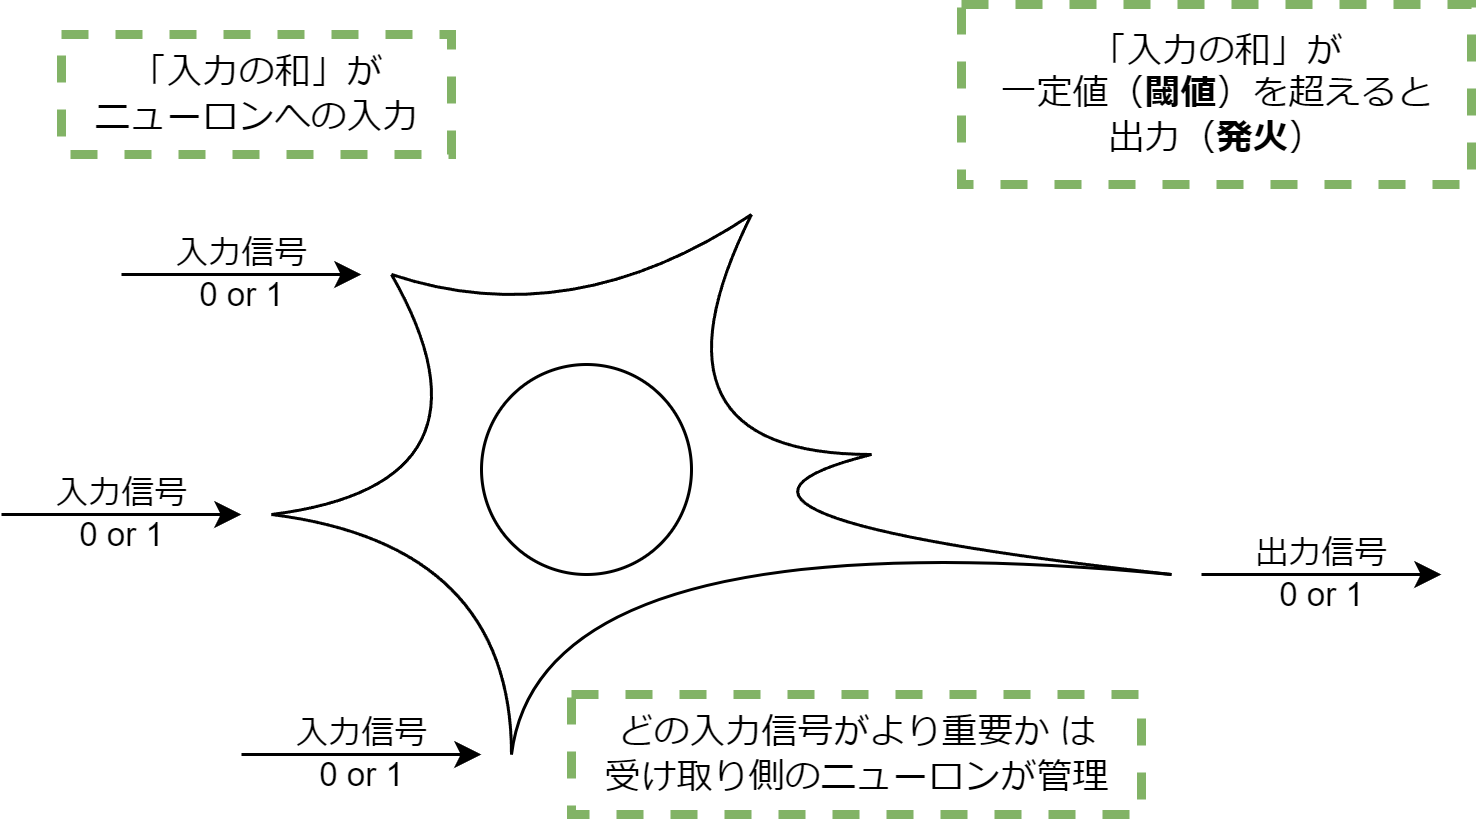
\includegraphics[width=0.6\linewidth]{img/ニューロンの働き}
		\end{figure}
	\end{frame}
	
	\subsection{ニューロンの働きの数理的解釈}
	\begin{frame}{ニューロンの働きの数理的解釈}
		\begin{figure}
			\centering
			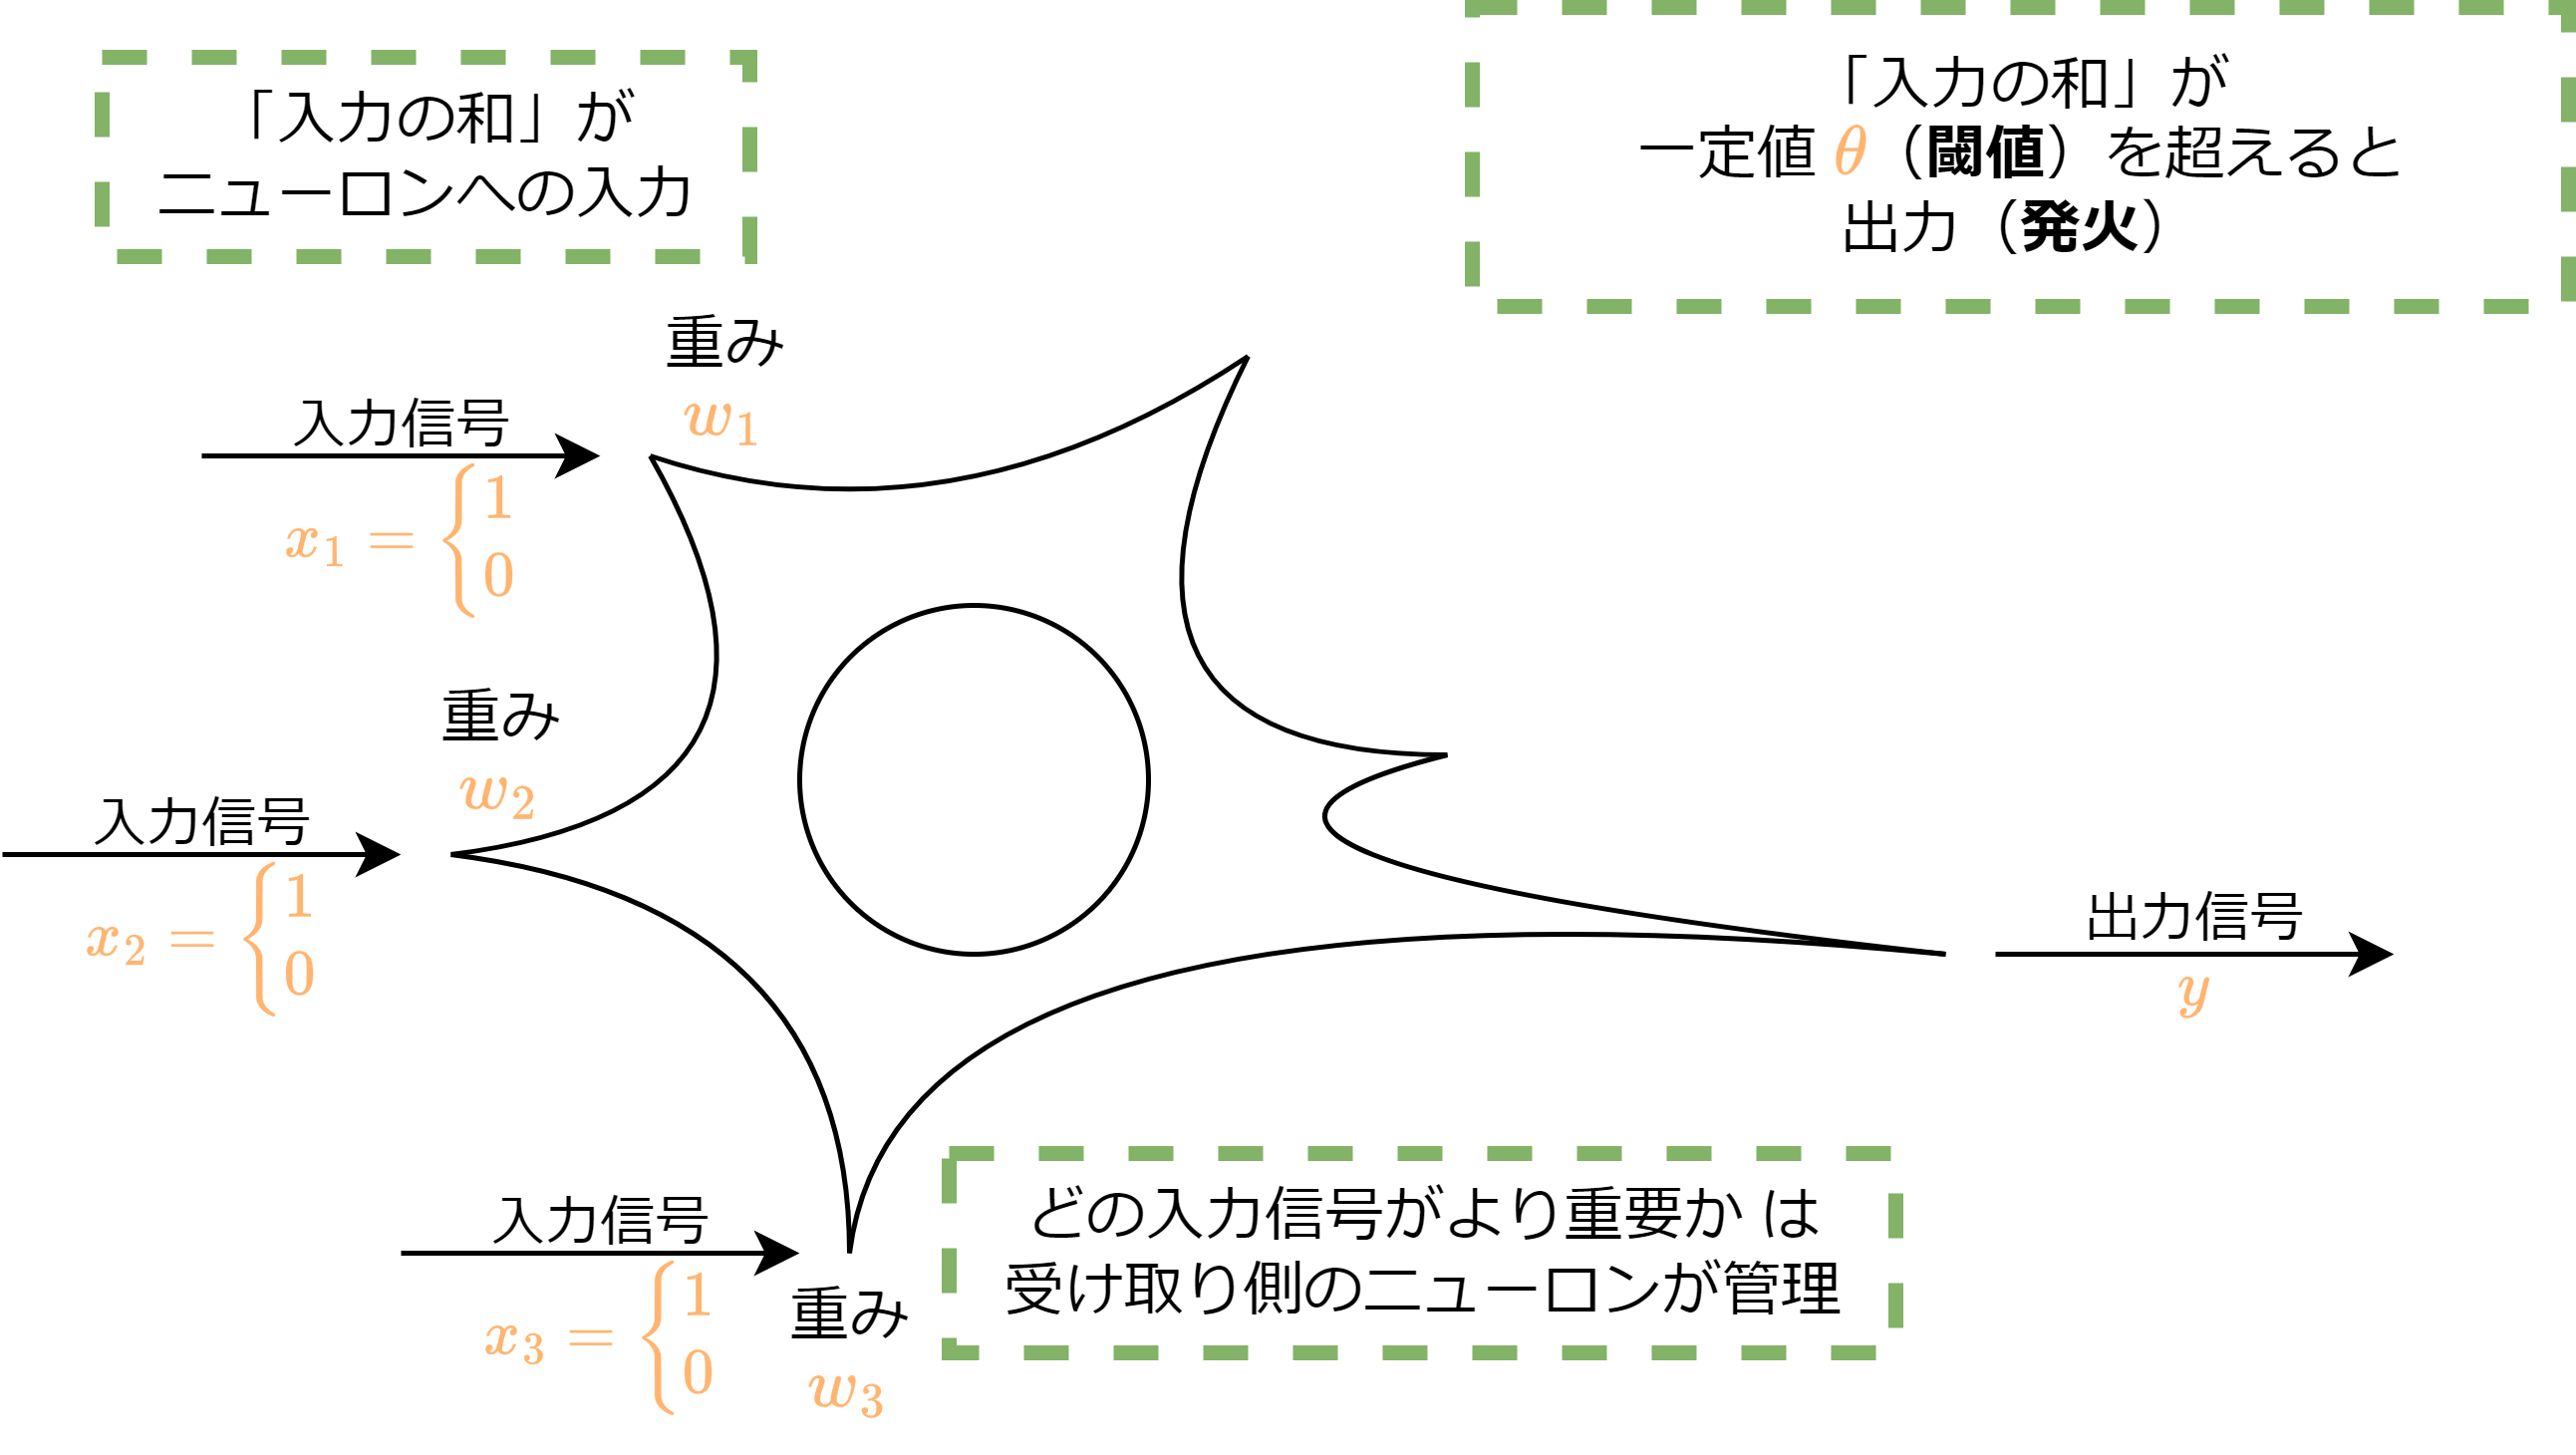
\includegraphics[width=0.7\linewidth]{img/ニューロンの数理的解釈}
		\end{figure}
		\begin{itemize}
			\item 出力信号なし($ y = 0 $):$ w_1x_1 + w_2x_2 + w_3x_3 < \theta $
			\item 出力信号あり($ y = 1 $):$ w_1x_1 + w_2x_2 + w_3x_3 \geq \theta $
		\end{itemize}
	\end{frame}
	\begin{frame}{発火の条件のグラフ表現}
		\begin{figure}
			\centering
			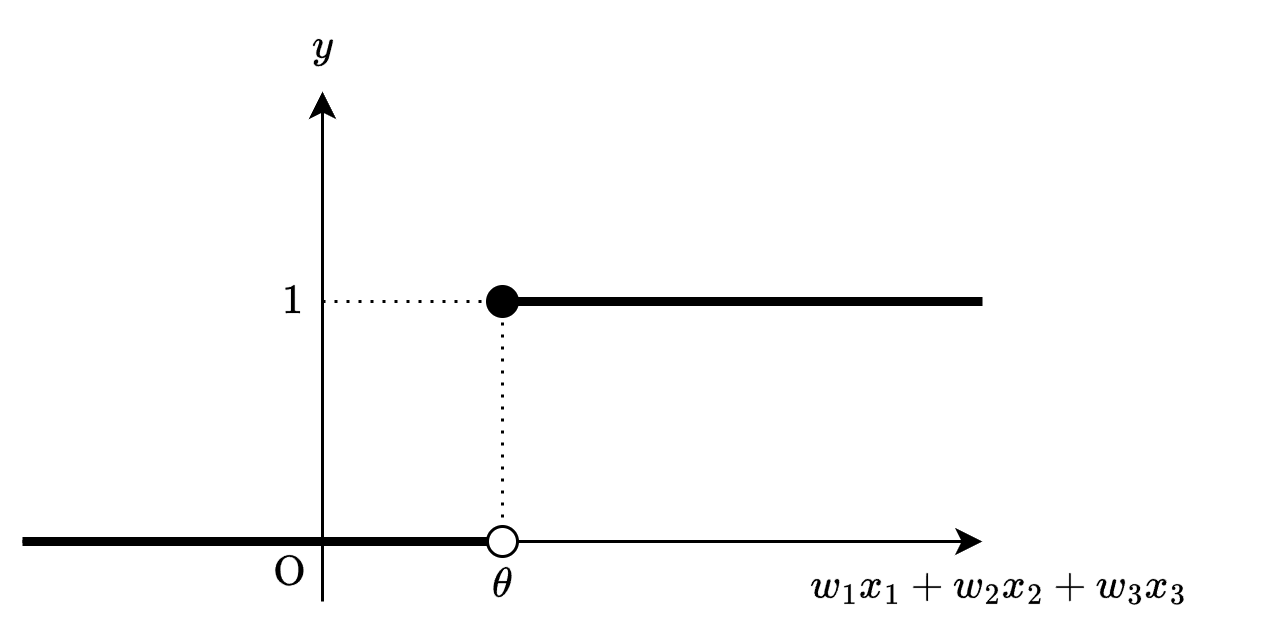
\includegraphics[width=0.9\linewidth]{img/発火の条件のグラフ}
		\end{figure}
	\end{frame}
	\begin{frame}{発火の式}
		\begin{itemize}
			\item 単位ステップ関数
		\end{itemize}
		\begin{figure}
			\centering
			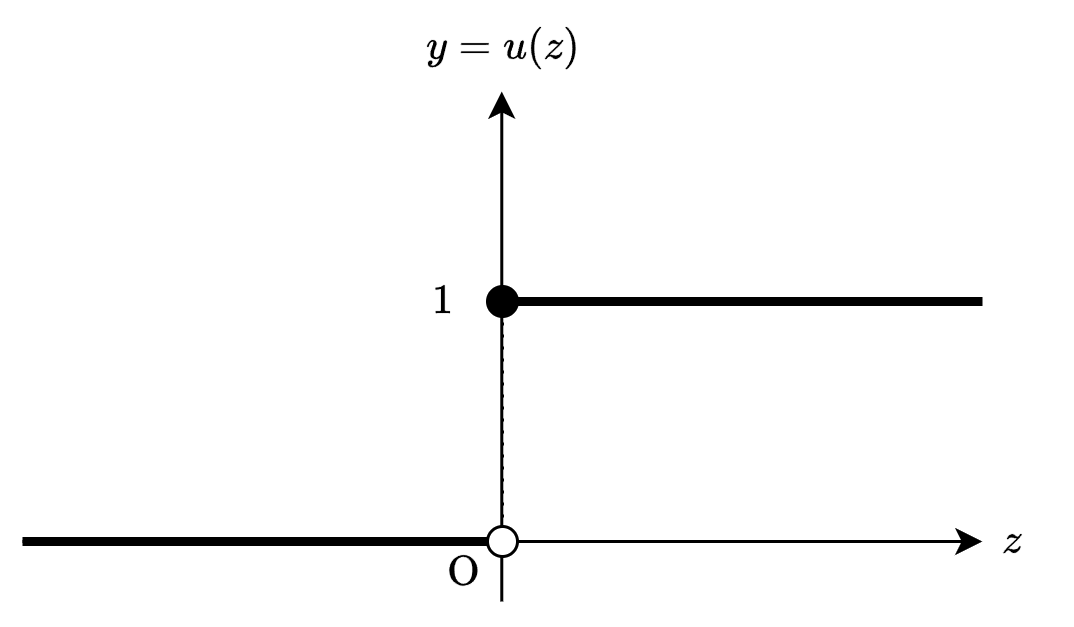
\includegraphics[width=0.5\linewidth]{img/単位ステップ関数}
		\end{figure}
		\begin{itemize}
			\item 発火の式:$ y = u(z) = u(w_1x_1 + w_2x_2 + w_3x_3 - \theta) $
			\begin{itemize}
				\item $ z = w_1x_1 + w_2x_2 + w_3x_3 - \theta $を、そのニューロンに対する\alert{重み付き入力}という
			\end{itemize}
		\end{itemize}
	\end{frame}
	\subsection{ユニット}
	\begin{frame}{ユニット}
		\begin{itemize}
			\item 簡略され抽象化されたニューロンを、生物学的なニューロンと区別して\alert{ユニット}(unit)とよぶ
		\end{itemize}
		\begin{figure}
			\centering
			
\includegraphics[width=0.7\linewidth]{img/ユニット}
		\end{figure}
	\end{frame}
	\begin{frame}{活性化関数}
		\begin{itemize}
			\item 発火の式(旧):$ y = u(w_1x_1 + w_2x_2 + w_3x_3 - \theta) $
			\begin{itemize}
				\item 単位ステップ関数$ u $に限定する必要はない
			\end{itemize}
			\item \alert{発火の式(新)}:$ y = a(w_1x_1 + w_2x_2 + w_3x_3 - \theta) $
			\begin{itemize}
				\item 関数$ a $を\alert{活性化関数}(activation function)という
				\item この関数$ a $はモデル作成者がさまざまに定義可能
			\end{itemize}
		\end{itemize}
	\end{frame}
	\begin{frame}{活性化関数の代表例}
		\alert{シグモイド関数}(Sigmoid function)
		\begin{equation*}
			\sigma(z) \triangleq \dfrac{1}{1 + e^{-z}}\quad (e = 2.71828\cdots)
		\end{equation*}
		\begin{figure}
			\centering
			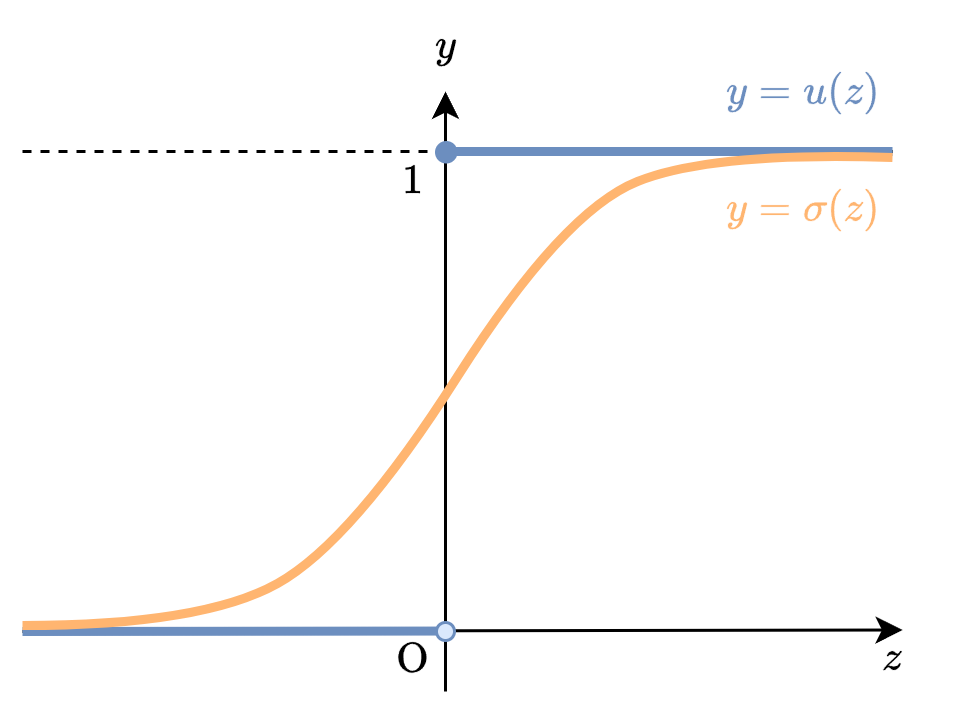
\includegraphics[width=0.5\linewidth]{img/単位ステップ関数とシグモイド関数}
		\end{figure}
	\end{frame}
	\begin{frame}{「発火の有無」から「興奮度」へ}
		\begin{figure}
			\centering
			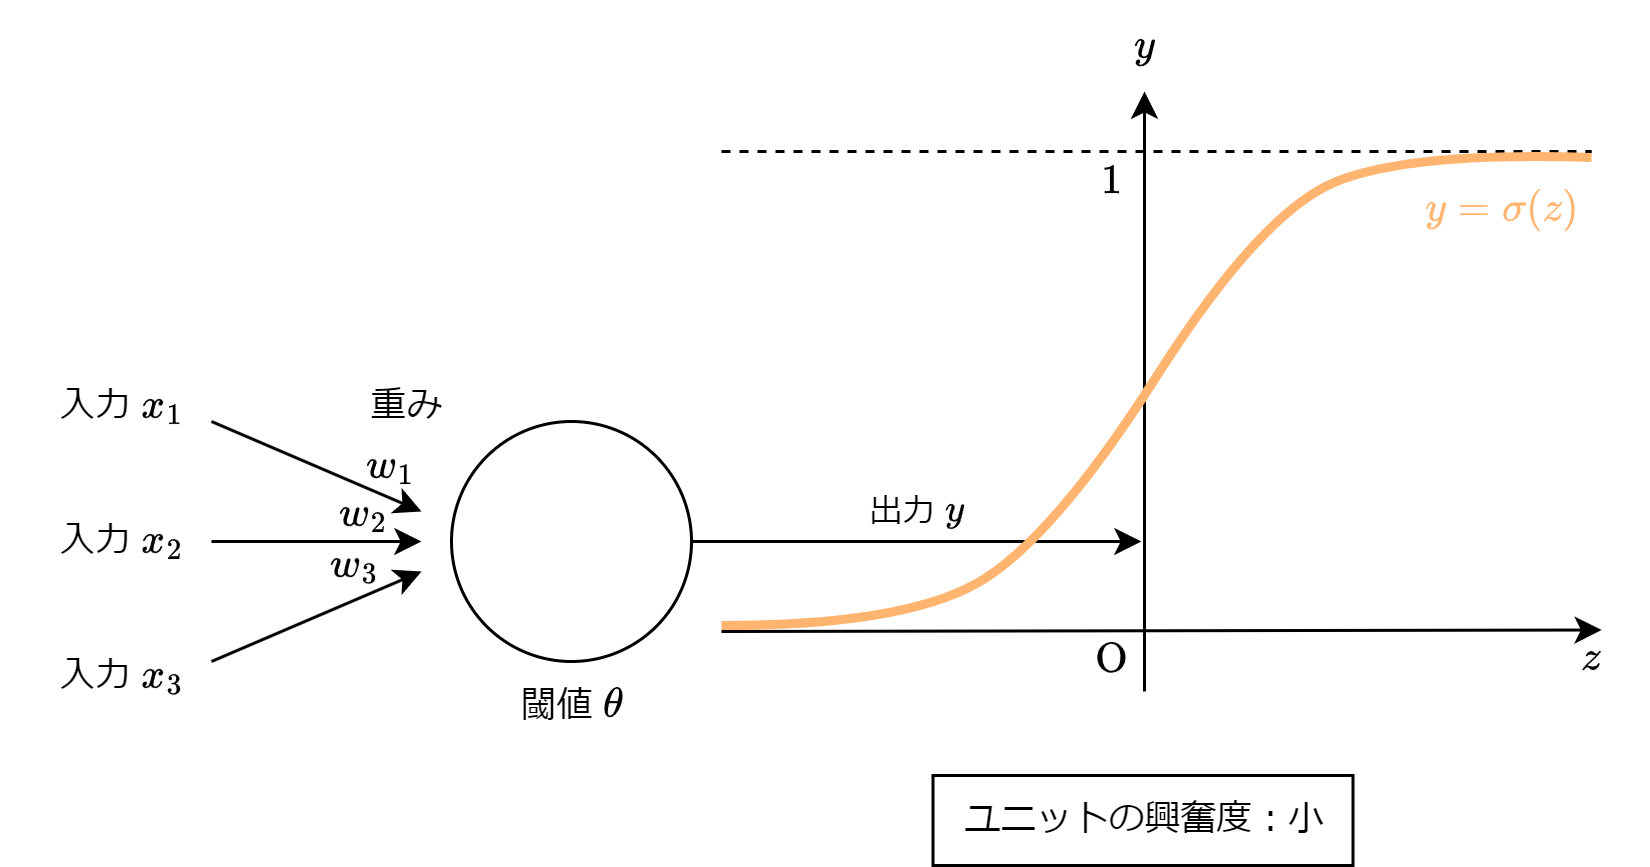
\includegraphics[width=0.8\linewidth]{img/ユニットの興奮度小}
		\end{figure}
		\begin{equation*}
			y = \sigma(w_1x_1 + w_2x_2 + w_3x_3 - \theta) 
		\end{equation*}
	\end{frame}
	\begin{frame}{「発火の有無」から「興奮度」へ}
		\begin{figure}
			\centering
			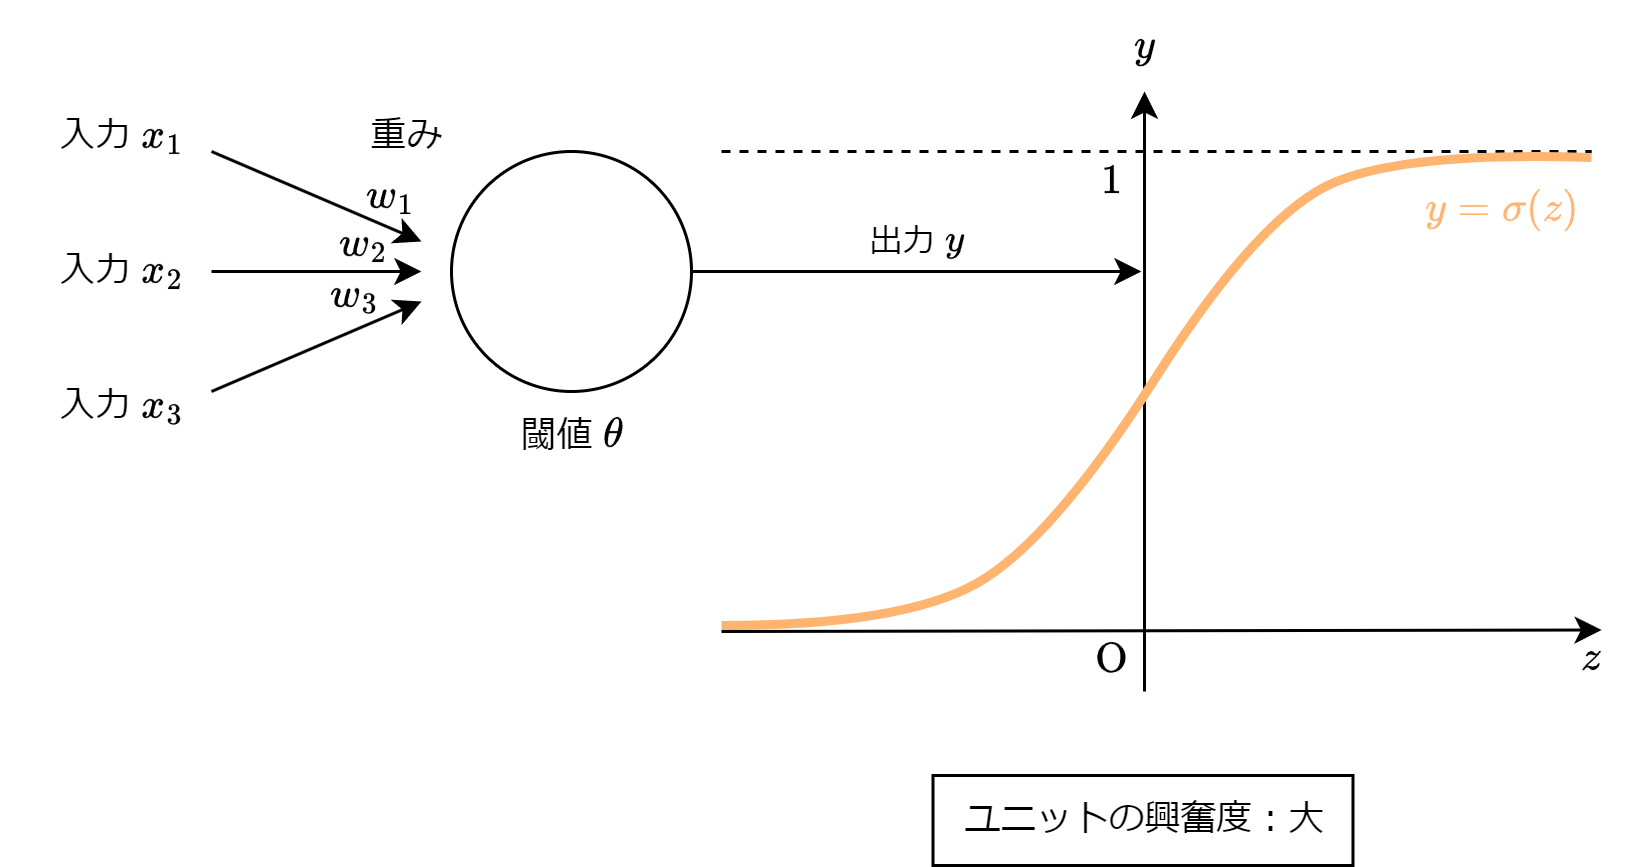
\includegraphics[width=0.8\linewidth]{img/ユニットの興奮度大}
		\end{figure}
		\begin{equation*}
			y = \sigma(w_1x_1 + w_2x_2 + w_3x_3 - \theta) 
		\end{equation*}
	\end{frame}
	\begin{frame}{バイアス}
		\sout{$ y = a(w_1x_1 + w_2x_2 + w_3x_3 - \theta) $}
		
		$ y = a(w_1x_1 + w_2x_2 + w_3x_3 + b) $		
		\begin{itemize}
			\item $ -\theta \longrightarrow +b $に表記を変更
			\item すべて足し算に統一することで計算しやすくなる
		\end{itemize}
	\end{frame}
	\begin{frame}{ユニットのまとめ}
		\begin{figure}
			\centering
			
\includegraphics[width=0.8\linewidth]{img/ユニットのまとめ}
		\end{figure}
		重み付き入力:$ z = w_1x_1 + w_2x_2 \cdots + w_nx_n + b $
		
		出力:$ y = \sigma(z) $
	\end{frame}

	\subsection{ニューラルネットワーク}
	\begin{frame}{ニューラルネットワーク(Neural Network; NN)}
		\begin{itemize}
			\item ユニットをネットワーク状に結合したもの
		\end{itemize}
		\begin{figure}
			\centering
			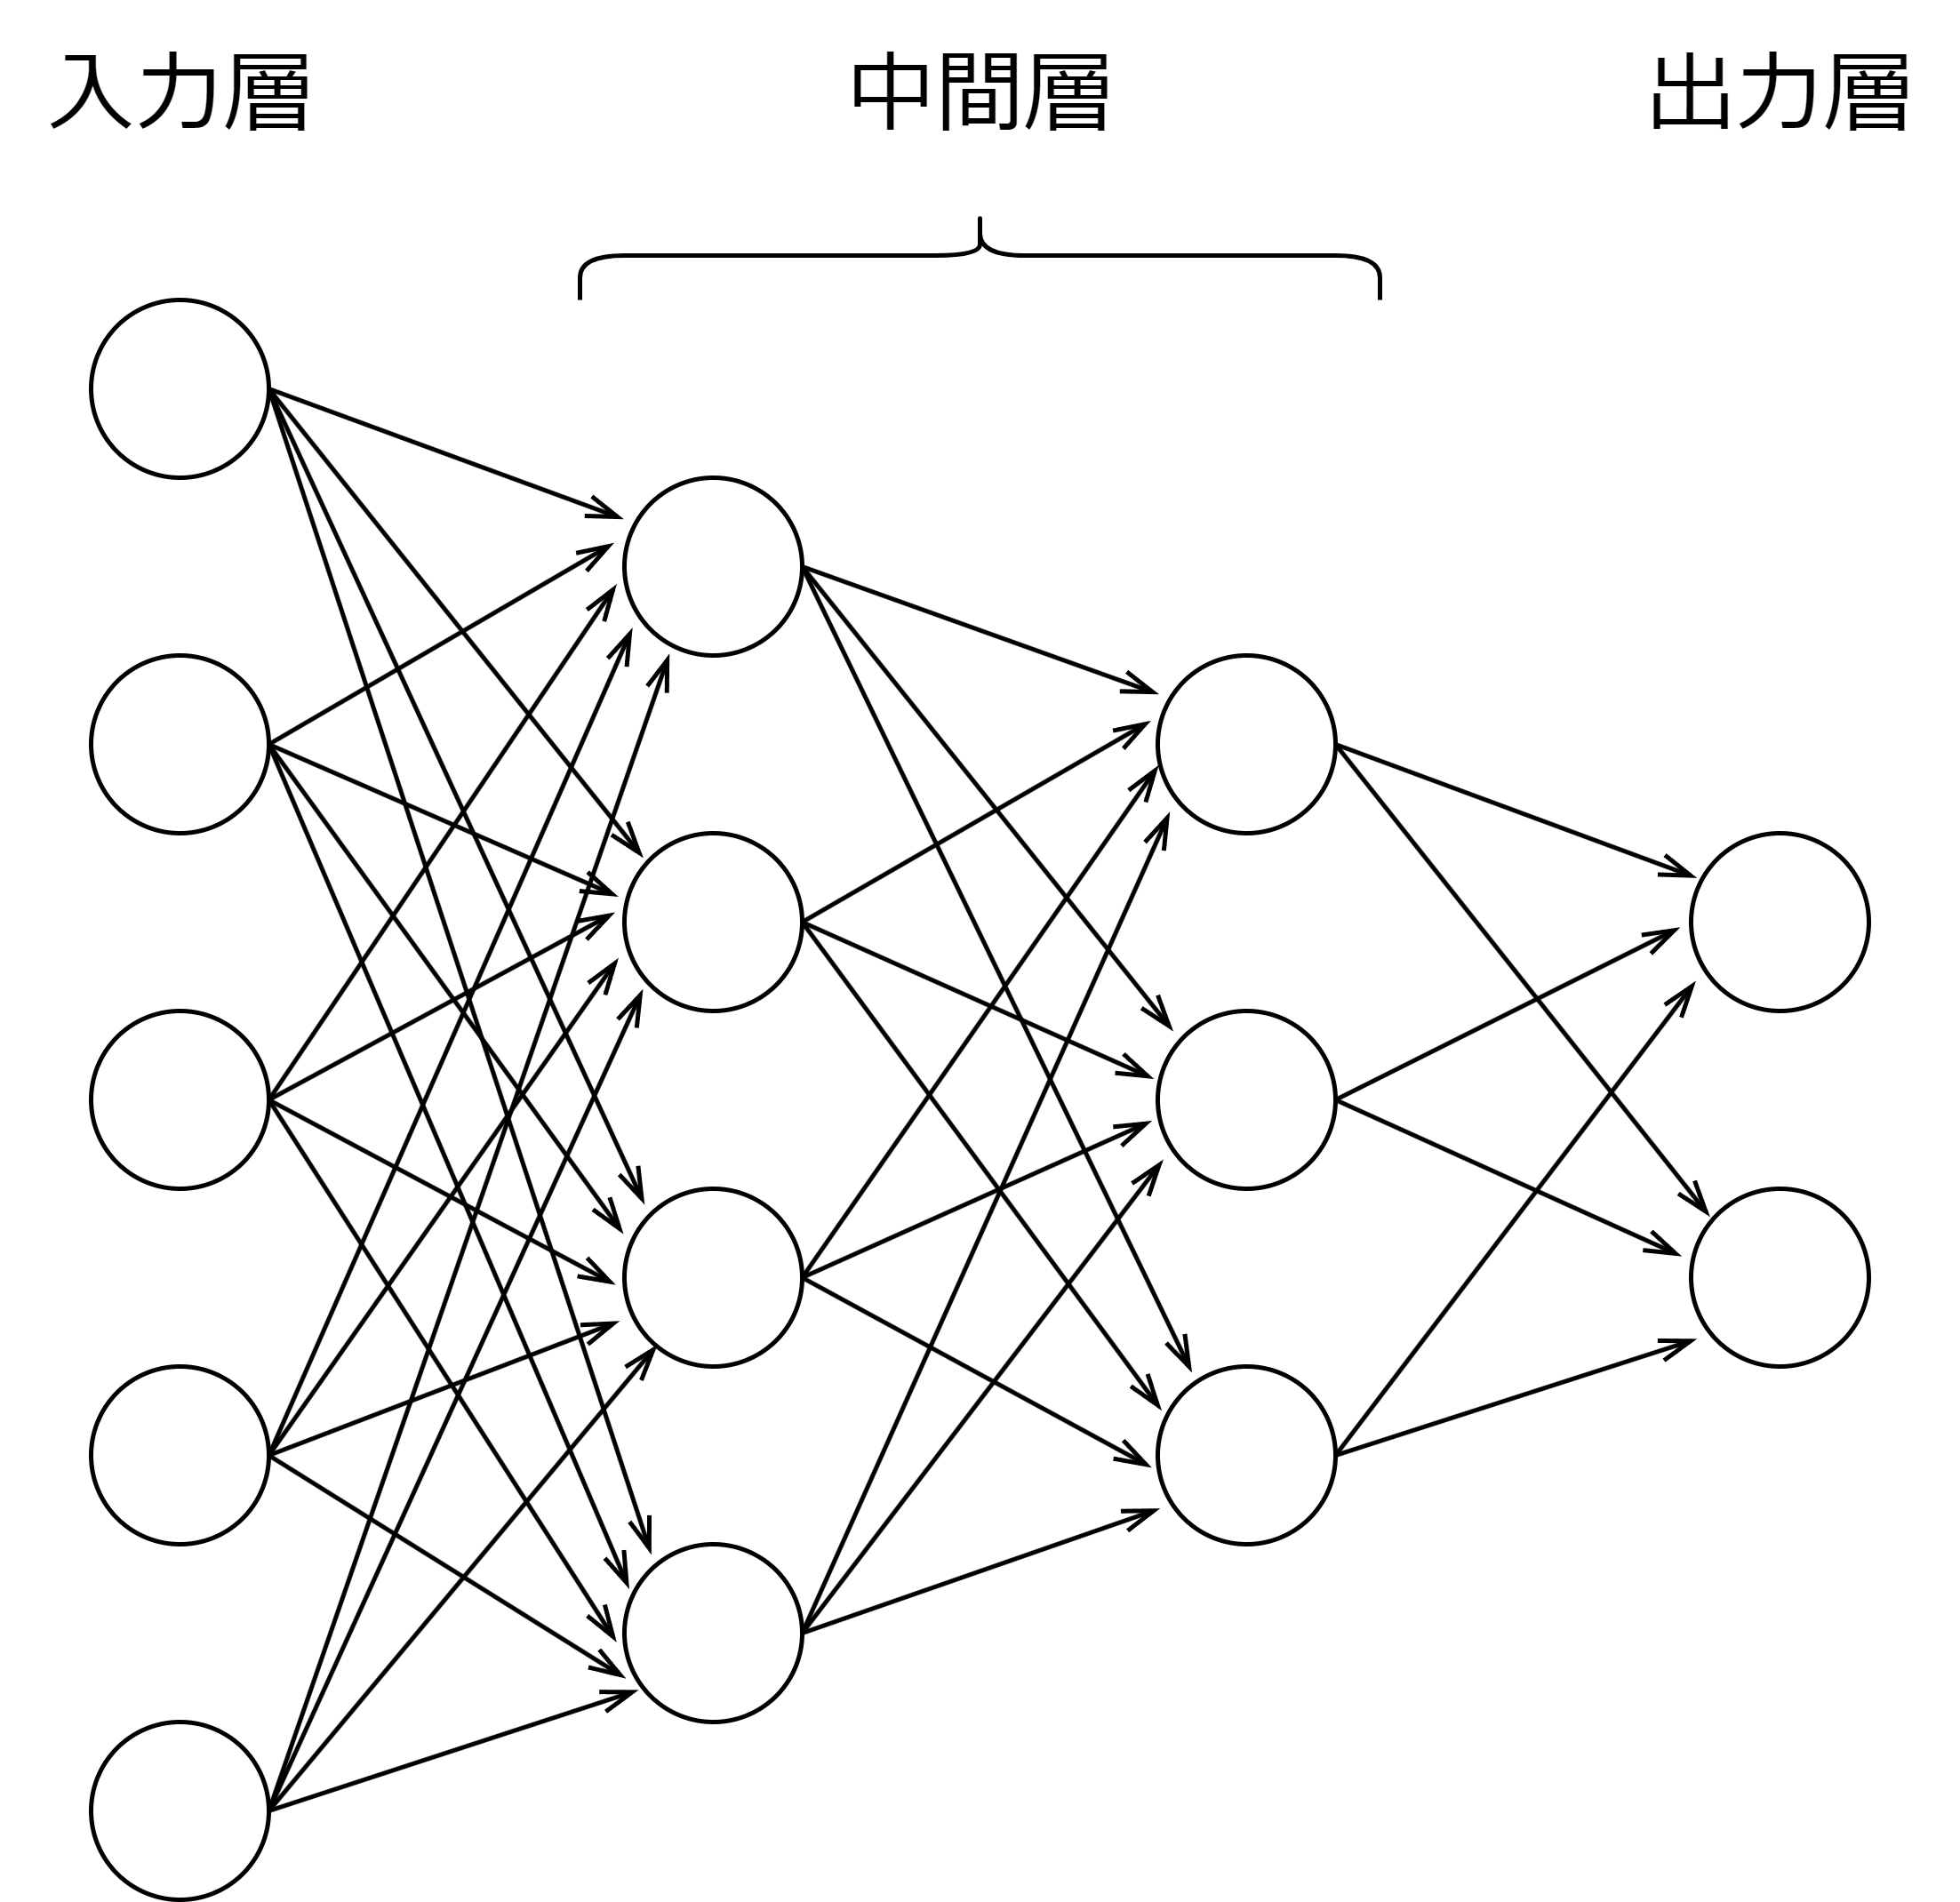
\includegraphics[width=0.4\linewidth]{img/階層型ニューラルネットワーク}
		\end{figure}
	\end{frame}
	\begin{frame}{ニューラルネットワークを用いた問題の具体例}
		\begin{block}{例題}
			$ 4 \times 3 $画素からなる画像で読み取られた手書きの数字「0」「1」を識別するニューラルネットワークを作成せよ。
			ただし、学習データは64枚の画像とし、画素はモノクロ2階調とする。
		\end{block}
		\begin{figure}
			\centering
			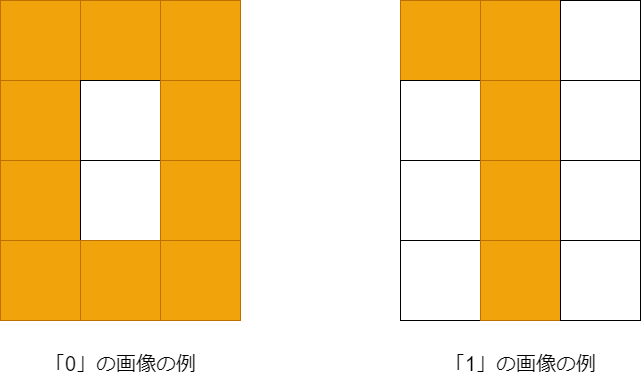
\includegraphics[width=0.5\linewidth]{img/0と1の画像の例}
		\end{figure}
	\end{frame}
	\begin{frame}{ニューラルネットワークを用いた問題の具体例}
		\underline{解答例}
		\begin{figure}
			\centering
			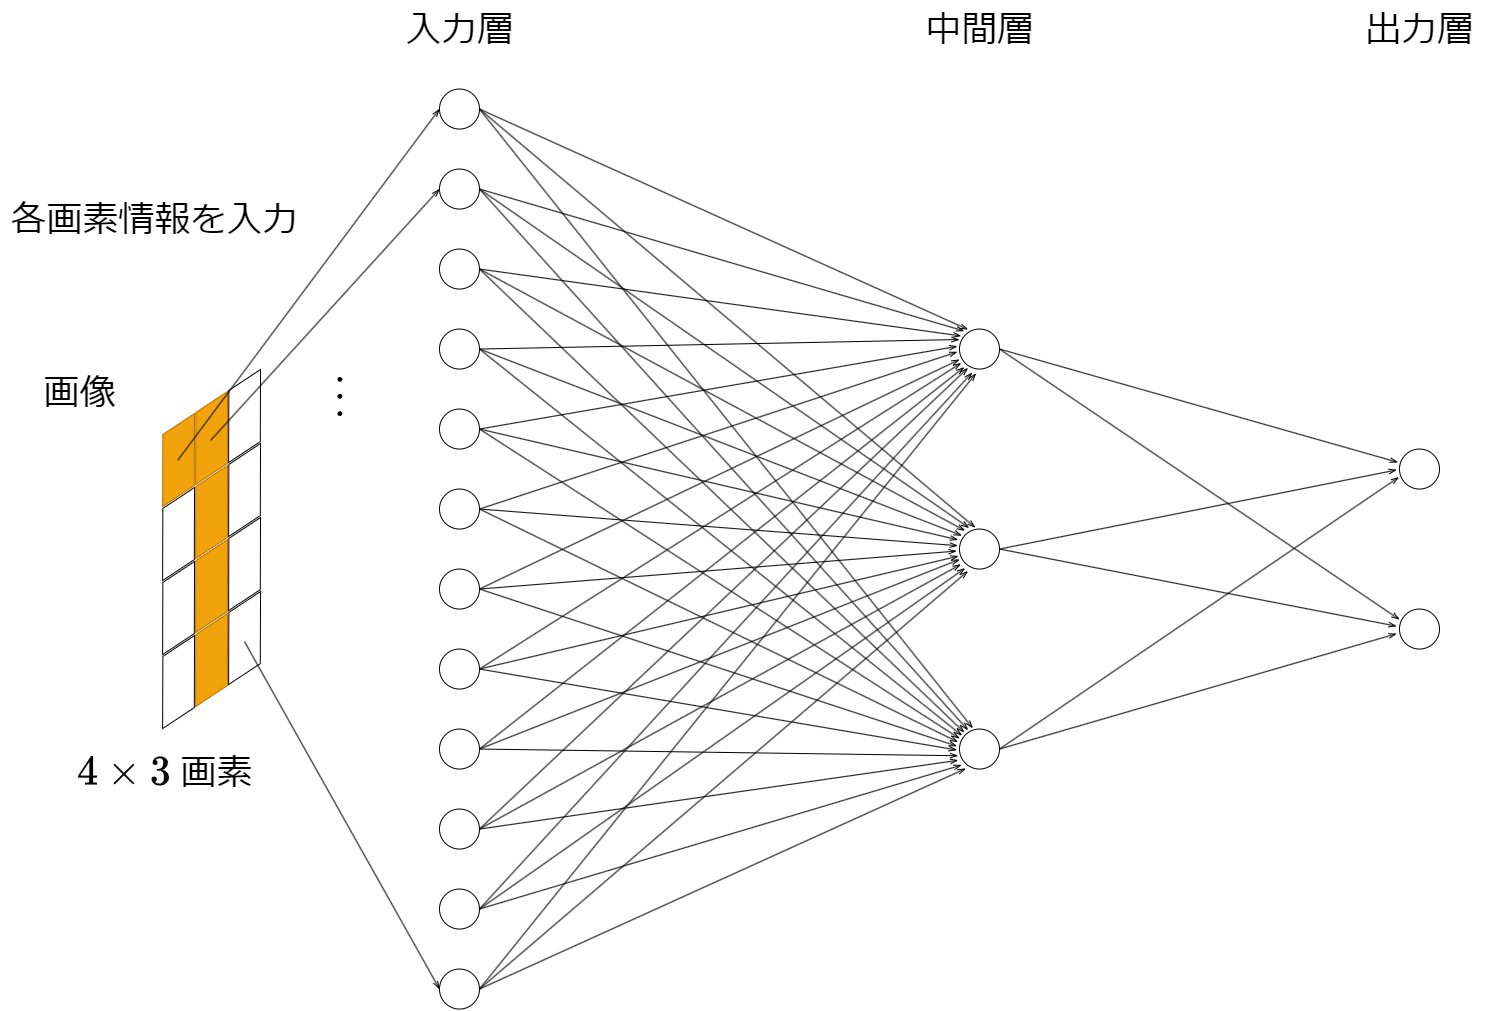
\includegraphics[width=0.6\linewidth]{img/具体的なニューラルネットワークの解答例}
		\end{figure}
	\end{frame}
\end{document}
